\documentclass{article}
\usepackage{tikz}
\usepackage{float}
\usepackage{amsmath}
\usepackage{lmodern}
\usepackage{amssymb}
\usetikzlibrary{calc}
\usetikzlibrary{hobby}
\usetikzlibrary{decorations.markings}
\usetikzlibrary{patterns, patterns.meta}
\usetikzlibrary{shapes}

\begin{document}


\centering

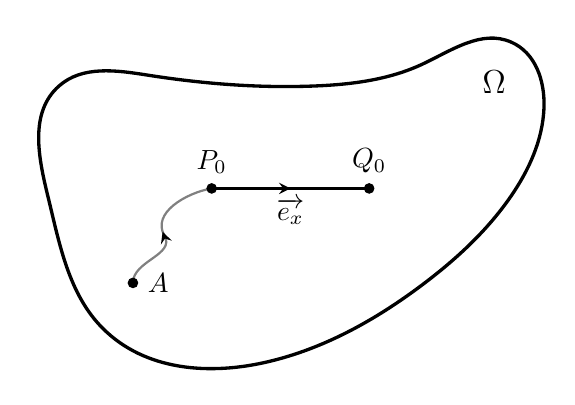
\begin{tikzpicture}
\pgfmathsetmacro{\CircleSize}{0.06}     % radius of coordinate circles/dots
% define styles used in this picture
\tikzset{
BigTextFont/.style={font=\large},
every node/.style={font=\normalsize, text=black},
CircleNodeStyle/.style={draw=black, shape=circle, fill=black, minimum size=\CircleSize*2 cm, inner sep=0pt},
arrowstyle/.style={->, >=stealth}}

% waypoint coordinates (in degrees, as seen from origin)
\begin{scope}[scale=1.4]
       \coordinate (10degrees) at (1.2,0.2);     
       \coordinate (25degrees) at (2.0,1.0); 
       \coordinate (35degrees) at (2.3,1.8);
       \coordinate (50degrees) at (2.0,2.4);
       \coordinate (60degrees) at (1.2,2.2);
       \coordinate (85degrees) at (0.2,2.0);
       \coordinate (120degrees) at (-1.3,2.1);
       \coordinate (135degrees) at (-2.1,2.0);
       \coordinate (155degrees) at (-2.2,1.0);
       \coordinate (185degrees) at (-1.7,-0.2);
       \coordinate (250degrees) at (-0.2,-0.5);
\end{scope}

% drawing area
\draw[postaction={decorate}, decoration={
       markings,
       mark=at position 0.23 with {\node[below, BigTextFont, inner sep=0.4cm] {$\Omega$};}}]
[very thick] (10degrees) to[closed, curve through =
{(25degrees) (35degrees) (50degrees) (60degrees) (85degrees) (120degrees) (135degrees) (155degrees) (185degrees) }] (250degrees);

% CHECK
%plotting the waypoints
%\foreach \c in {(Odegrees),(20degrees),(40degrees),(55degrees),(80degrees),
%(95degrees),(110degrees),(180degrees),(260degrees),(300degrees),(330degrees)} \fill[red] \c circle (1.0mm);

% coordinates (P0, Q0 and A)
\coordinate (P0) at (-1.0, 1.5);
\coordinate (Q0) at ($(P0)+(2.0,0)$);
\coordinate (A) at ($(P0)+(-1.0,-1.2)$);

% path P0 -> Q0
\draw[postaction={decorate}, decoration={
       markings,
       mark=at position 0.50 with {\node[below] {$\overrightarrow{e_x}$};},
       mark=at position 0.50 with {\arrow{stealth}}}]
[thick] (P0) -- (Q0);

% path A -> P0
\coordinate (AP1) at ($(A)+(0.4,0.6)$);
\coordinate (AP2) at ($(P0)+(-0.2,-0.4)$);
\draw[postaction={decorate}, decoration={
       markings,
       mark=at position 0.475 with {\arrow[black]{stealth}}}]
[thick, gray] (A) to[out=90, in=300] (AP1) to[out=120, in=190] (P0); 

% nodes (P0, Q0 and A)
\node [CircleNodeStyle, label=above:$P_{0}$] at (P0) {};
\node [CircleNodeStyle, label=above:$Q_{0}$] at (Q0) {};
\node [CircleNodeStyle, label=right:$A$] at (A) {};

\end{tikzpicture}

\end{document}
